\chapter{Bolometri}
In fisica delle particelle, il bolometro \`e un dispositivo in grado di rivelare particelle mediante misure di calore;
esso viene spesso usato per la misura ad alta risoluzione di eventi rari.
In questi dispositivi l'informazione sull'energia viene portata dai fononi del reticolo cristallino: quando una particella
incide sul bolometro, la sua energia viene convertita in calore che viene misurato.
\section{Struttura di base di un bolometro}
La struttura di base di un bolometro \`e in figura~\ref{fig:strutturaBolometro}, in particolare in prima approssimazione
si pu\`o pensare il bolometro come un dispositivo formato da un assorbitore di capacit\`a termica C ed un sensore di sensibilit\`a A accoppiati
ad un bagno termico a temperatura $T_0$ mediante un conduttore di conducibilit\`a G.
Inoltre, in prima approssimazione, si pu\`o pensare che il sensore e l'assorbitore siano accoppiati da una conducibilit\`a termica elevata tale
per cui sono costantemente in equilibrio termico.
\begin{figure}[htbp]
\begin{center}
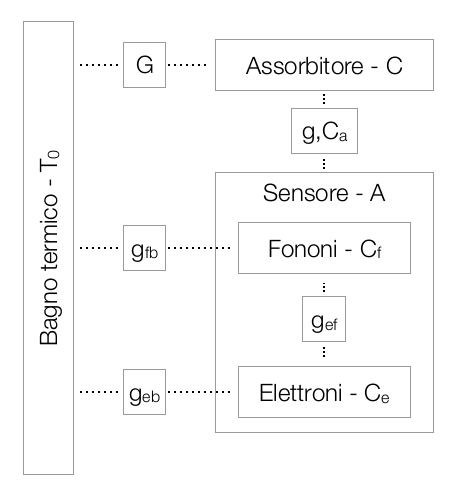
\includegraphics[scale=1]{./Immagini/StrutturaBolometro.png}
\caption{Struttura di base di un bolometro}
\label{fig:strutturaBolometro}
\end{center}
\end{figure}
Supponiamo che una particella di energia $E$ incida sull'assorbitore: interagendo con esso, vi deposita tutta l'energia che dopo un tempo nell'ordine
dei ns diventa calore.
\`E possibile, quindi, associare un aumento di temperatura proporzionale all'energia secondo:
\begin{equation*}
\Delta T = \frac{Q}{C_T}
\end{equation*}
Nei bolometri si cerca di avere $C_T$ minori possibili, in modo da avere aumenti di temperatura grandi e facilmente misurabili;
un termometro si occupa di misurare tali variazioni e produce un segnale elettrico che sia proporzionale.
Il calore fluisce, mediante G, verso il bagno termico che riporta l'assorbitore alla temperatura iniziale dopo un certo tempo $\tau=C/G$; il bagno termico deve avere una capacit\`a
termica elevata, per fare in modo di non variare troppo la propria temperatura assorbendo il calore.
\section{Evoluzione di un segnale di un bolometro}
Il bolometro pu\`o essere visto in modo semplificato come il circuito elettrico in figura~\ref{fig:circuitoBolometro}:
in seguito al passaggio della particella, un flusso di calore $P_{in}$ entra nel circuito RC con $R=G^{-1}$ e $C=C_T$; ai capi della capacit\`a
\`e presente una differenza di temperatura che viene misurata dal termometro.
\begin{figure}[htbp]
\begin{center}
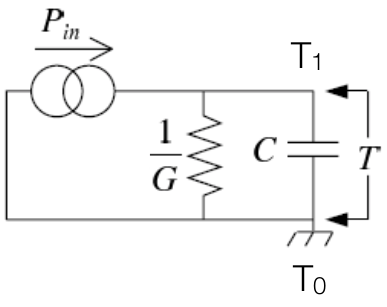
\includegraphics[scale=0.50]{./Immagini/CircuitoBolometro.png}
\caption{Rappresentazione circuitale di un bolometro}
\label{fig:circuitoBolometro}
\end{center}
\end{figure}
Il flusso di calore ha lo stesso ruolo della corrente elettrica: 
\begin{equation*}
P_{in} = \delta(T)E = G(T_1 - T_0) + C \frac{dT_1}{dt}
\end{equation*}
dove si introduce una delta di Dirac approssimando che tale energia venga prodotta istantaneamente.
Risolvendo si trova:
\begin{equation*}
T_1 = \frac{E}{C}e^{-t/\tau} + T_0
\end{equation*}
con $\tau=C/G$, come in un RC.\\
\section{Fononi in un bolometro}
Quando una particella deposita energia nel bolometro, vengono eccitati i fononi atermici, essi dopo poco tempo vengono termalizzati tramite diffusioni
nel reticolo cristallino.
\begin{figure}[htbp]
\begin{center}
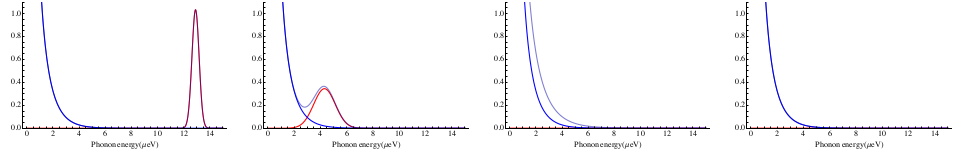
\includegraphics[scale=0.45]{./Immagini/SpettroFononi.png}
\caption{Andamento temporale dello spettro dei fononi in un cristallo}
\label{fig:spettroFononi}
\end{center}
\end{figure}
La figura~\ref{fig:spettroFononi} mostra l'andamento dello spettro, le prime due fasi avvengono in tempi nei $\mu$s, la misurazione di tale spettro
porta a misure a bassa risoluzione di energia, di posizione con buona risoluzione spaziale e del tipo di radiazione.
Le altre due fasi avvengono in tempo tra i $\mu$s e i s e permettono di ottenere misure ad alta risoluzione di energia e tipo di particella.
\section{Risoluzione energetica nei bolometri}
Alle temperatura di lavoro dei bolometri, i fononi termici hanno energie nei $\mu$eV, permettendo di ottenere ottime risoluzioni energetiche.
Il numero di fotoni vale:
\begin{equation*}
N \propto \frac{C(T)}{k_B}
\end{equation*}
per cui:
\begin{equation*}
\Delta E = \Delta N <E>  = \sqrt{\frac{C(T)}{k_B}}\, k_B T = \frac{C(T) k_B T^2} \sim 10 \text{eV a 1 MeV}
\end{equation*}
Essa non dipende dall'energia incidente, bensi dalla capacit\`a e pi\`u che quadraticamente dalla temperatura.\\
Nella realt\`a sulla risoluzione incidono altri fattori che contribuiscono a peggiorarla, ad esempio nell'esperimento CUORE la risoluzione \`e
di 5 keV, con noise a 500 eV.
Effetti che incidono sulla risoluzione sono imperfezioni del cristallo, scintillazioni, effetti di superficie e conduttanze termiche parassite che disperdono calore.\\
I microbolometri riescono a misurare keV con la precisione dei mev.
\section{L'assorbitore}
L'assorbitore determina il processo fisico che verr\`a studiato nel bolometro.
Esso viene scelto in base alle particelle che voglio rivelare, \`e possibile scegliere il materiale in modo che sia esso stesso sorgente dell'evento che
voglio studiare. 
La scelta del materiale ha ampie libert\`a, \`e possibile utilizzare materiali scintillanti, liquidi, semiconduttori...
Il materiale viene tipicamente scelto con una capacit\`a termica molto piccola; il sensore pu\`o essere all'interno (rivelatore monolitico)
o all'esterno (rivelatore composito).
I macrobolometri hanno capacit\`a termiche pi\`u grandi con masse nei g e dimensioni nei cm, i microbolometri hanno masse nei mg e dimensioni nei
$\mu$m.\\
La capacit\`a termica deve essere piccola per avere variazioni misurabili di temperatura e ottime risoluzioni energetiche.
Tipicamente si cerca di usare dielettrici e diamagnetici, in quanto i gradi di libert\`a dovuti ai campi aumentano la capacit\`a.
Alla fine per\`o siccome la capacit\`a diminuisce con la temperatura al cubo, basta che un materiale sia abbastanza freddo per fungere da bolometro,
da qui la grande libert\`a di scelta nel materiale.
\section{Il sensore}
I sensori misurano l'energia, il tipo di particella, la posizione e il momento; questi dispositivi hanno una qualche
propriet\`a fisica dipendente dalla temperatura, misurandone la variazione si ricava la temperatura del bolometro.
\subsection{Semiconductor Thermistors}
Sono chip di silicio e germanio drogati, la loro resistivit\`a dipende dalla temperatura secondo
\begin{equation*}
\rho(T) = \rho_0 e^{-t/T_0}
\end{equation*}
con $\rho_0$ e $T_0$ dipendenti dal drogaggio.
La sensibilit\`a logaritmica del dispositivo \`e definita come:
\begin{equation*}
A = \frac{d\text{log}(R(T))}{d\text{log}(T)} = 1 - 10
\end{equation*}
La resistenza viene misurata mediante un partitore resistivo.
Il punto pi\`u interessante di lavoro \`e la regione di feedback elettrotermico (figura~\ref{fig:feedbackElettrotermico}), in questa
zona la resistenza \`e estremamente sensibile alle variazioni di temperatura.
\begin{figure}[htbp]
\begin{center}
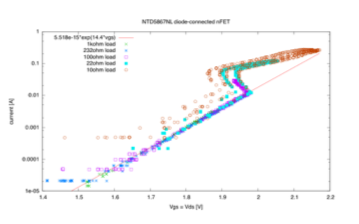
\includegraphics[scale=1]{./Immagini/FeedbackElettrotermico.png}
\caption{Curva di lavoro di un ST}
\label{fig:feedbackElettrotermico}
\end{center}
\end{figure}
Generalmente il germanio viene drogato mediante l'impiantazione di neutroni, questo permette di avere un piccola capacit\`a termica per via dell'elevata
intrinsecit\`a del cristallo.
Il silicio \`e pi\`u semplice da produrre ed \`e ampiamente utilizzato, ha una sensibilit\`a inferiore e viene utilizzato nei microbolometri.\\
Questi termometri hanno il vantaggio di avere un utilizzo semplice, un'alta impedenza (permette elettronica non spinta) e hanno un 
buon range dinamico. 
Il problema \`e che sono soggetti a microfonismo e hanno volumi non trascurabili (si pu\`o perdere energia all'interno).
Questi dispositivi sono insensibili ai fononi atermici.
\subsection{Transition Edge Sensors (TES)}
I TES utilizzano semiconduttori intorno alla temperatura di transizione, in queste condizioni, infatti, la dipendenza della resistenza dalla temperatura \`e fortissima,
per cui i dispositivi che misurano tale resistenza sono estremamente sensibili alle variazioni di temperatura (nel mK) (fig.~\ref{fig:TES}).
\begin{figure}[htbp]
\begin{center}
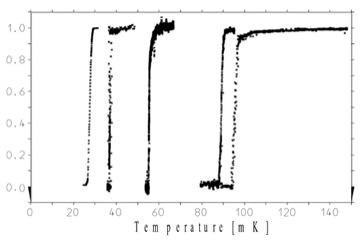
\includegraphics[scale=1]{./Immagini/TES.png}
\caption{Transizione in un superconduttore}
\label{fig:TES}
\end{center}
\end{figure}
Sul bolometro viene depositato un film ($\sim 100$ nm) di superconduttore che misura i fononi che termalizzano al suo interno.
Questi dispositivi hanno una sensibilit\`a logaritmica intorno a 1000, inoltre la loro risposta \`e estremamente veloce, permettendo di
misurare i fononi atermici.
I principali difetti di questi termometri sono legati al range dinamico stretto e alla loro bassa impedenza, che richiede elettronica
dedicata.
\subsection{Altri termometri}
\begin{itemize}
\item \textbf{Magnetic Micro Calorimeters}, sfruttano la dipendenza dalla temperatura della magnetizzazione
\item \textbf{Microwave Kinetic Inductance Detectors}, lavorano sulla variazione di induttanza
\item \textbf{Superconductive Tunnel Junctions}, misurano la corrente generata per effetto tunnel dalla rottura di coppie di Cooper
\end{itemize}
\section{Il bagno termico}
I bolometri devono funzionare a bassa temperatura per ottenere la massima risoluzione energetica e ampiezza del segnale, per questo
sono collegati a bagni termici che si occupano di mantenerli a bassa temperatura.
Tipicamente questi dispositivi lavorano a temperature nei 100 mK (per i microbolometri) o 10 mK per i macrobolometri, in particolare
questi ultimi lavorano a temperature pi\`u basse perch\`e hanno capacit\`a termiche maggiori rispetto ai micro.
I segnali prodotti nei bolometri sono nell'ordine dei 10 - 100 $\mu$K, per cui \`e necessario che si abbiano temperature stabili fino a $10^{-5} \mu$K,
il sistema che toglie il calore deve essere, quindi, efficiente e stabile.
Nei bolometri si utilizzano criostati con \textbf{unit\`a a diluizione}.\\
I criostati sono dispositivi formati da volumi a schemi concentrici (a cipolla), tra un volume e l'altro \`e presente del vuoto che minimizza
la convezione e la conduzione. 
Gli strati sono a temperature gradualmente decrescenti, per minimizzare l'irraggiamento, mentre nella parte interna \`e presente una regione
che attivemente rimuove il calore, nel caso del bolometro l'unit\`a a diluizione, l'unica che \`e in grado di poter portare oggetti a temperature
nei mK.
\subsection{L'unit\`a a diluizione}
L'unit\`a a diluizione \`e formata da una miscela di $^3\text{He}$ e $^4$He, quando si portano le temperature ad un punto sufficientemente basso (meno di 1 K)
l'elio si divide in due fasi, una concentrata e una diluita: nella fase diluita l'elio-3 (fermione) si scioglie all'interno dell'elio-4 (bosone che diventa superfluido).
A basse temperature l'elio-3 va in fase concentrata (simile ad un liquido) e l'elio-4 diventa superfluido, a temperature pi\`u alte l'elio-3 passa
alla fase diluita (simile ad un gas) e si discioglie nell'elio-4.
Questo processo \`e simile ad un evaporazione, dunque ha un proprio calore latente in quanto endotermico, per questo \`e in grado di portare via calore.\\
Nella pratica questo avviene pompando la miscela in un volume suddiviso in due regioni, la mixing chamber e lo still (fig.~\ref{fig:unitaDiluizione}).
Nello still l'elio-3 viene pompato via e continua ad evaporare per via della pressione di vapore saturo bassissima, l'evaporazione
induce il passaggio dalla fase concentrata alla diluita all'interno della mixing chamber, che refrigera.
L'elio-3 pompato via viene fatto ricondensare e reinserito nella mixing chamber, tenendo attivo il ciclo.
\begin{figure}[htbp]
\begin{center}
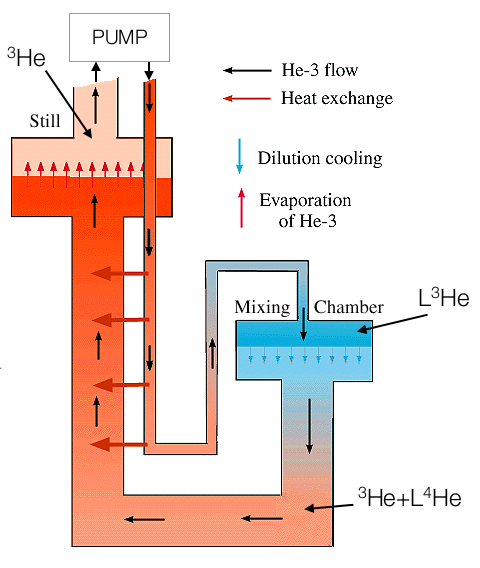
\includegraphics[scale=0.50]{./Immagini/UnitaDiluizione.png}
\caption{Funzionamento schematico di un'unit\`a a diluizione}
\label{fig:unitaDiluizione}
\end{center}
\end{figure}
L'elio \`e l'unico gas utilizzabile per questo processo, in quanto \`e ancora gassoso alle temperature di operazione.\\
Un piatto di rame collega il bolometro alla mixing chamber, in particolare tra il piatto e il bolometro \`e presente del teflon per fornire un
minimo di isolamento (per misurare il segnale che altrimenti sparirebbe subito).
\section{Confronto con gli altri rivelatori}
Il grande vantaggio dei bolometri \`e nell'elevatissima risoluzione, nella flessibilit\`a nella scelta dei materiali e della massa, inoltre non hanno
strati morti che assorbono energia.
Gli svantaggi sono nella difficile costruzione e impiego, nel tempo lento di risposta e nella sensibilit\`a al fondo ambientale.
\section{Impiego}
I bolometri sono impiegati nello studio di fenomeni rari (neutrini, in pratica). 
Essi sono stati utilizzati per studiare i decadimenti doppio beta con neutrino e ora sono impiegati nella ricerca del decadimento doppio beta senza neutrini.
Vengono anche impiegati per lo studio di decadimenti beta singoli, per lo studio della massa dei neutrini.
